\documentclass[12pt]{article}
\usepackage[a4paper, margin=1in]{geometry} 
\usepackage{graphicx} 
\usepackage{hyperref}
\usepackage{float}
\usepackage{multicol}
\usepackage[font=small, labelfont=bf]{caption}

\title{Lecture Notes for \\ INF281 Basics of Bioinformatics Sequence Analysis}
\author{Takaya Saito}
\date{}

\begin{document}

\pagenumbering{arabic}
\setcounter{page}{8}

\makeatletter 
\renewcommand{\thefigure}{\arabic{section}.\arabic{figure}}
\renewcommand{\thetable}{\arabic{section}.\arabic{table}}
\makeatother

%
% PART II
%
\setcounter{part}{1}
\part{}

%
% Global_pairwise_alignment
%
\setcounter{section}{1}
\setcounter{figure}{0}
\section{Global pairwise alignment}
%\documentclass[12pt]{article}
%\usepackage[a4paper, margin=1in]{geometry} 
%\usepackage{graphicx} 
%\usepackage{hyperref}
%\usepackage{float}
%\usepackage{multicol}
%\usepackage[font=small, labelfont=bf]{caption}
%
%\begin{document}

%
% Pairwise alignment
%
\subsection{Pairwise alignment}
A pairwise alignments is a basic sequence structure that consits of two sequences. A global alignment stretches to the whole part of two sequences, whereas a local alignment usually contains only part of the sequences.

%
% Pairwise alignment
%
\subsubsection*{Components of pairwise alignment}

We name two sequences as ‘database’ or ‘d’ and ‘query’ or ‘q’ through this course. They may represent sequences from two different species or organisms.
\\

\noindent
Identical sequences.
\begin{verbatim}
    q: ACGT
    d: ACGT
\end{verbatim}

\noindent
One mismatch.
\begin{verbatim}
    q: ACGT
    d: ACGA
\end{verbatim}

\noindent
The '-' symbol represents a blank. A single or a set of multile blanks further reprents a gap, which is an indication of insertion or deletion in the course of evoluation between two organisms.
\begin{verbatim}
    q: ACGT
    d: A-GT
\end{verbatim}

\noindent
\textbf{N.B.} A gap cannot be aligned with another gap.

%
% Example of a simple scoring scheme
%
\subsubsection*{Example of a simple scoring scheme}
\begin{itemize}
\item Match: 1
\item Mismatch: 0
\item Gap penalty: 1 (use -1 for the actual calculation)
\end{itemize}

\noindent
We may use the following notation.
\begin{itemize}
\item $R_{ab}$ = 1 for a = b
\item $R_{ab}$ = 0 for a $\neq$ b
\item g = 1
\end{itemize}

%
% NEW PAGE
%
\newpage 

%
% Exercise \thesection.1
%
\subsubsection*{Exercise \thesection.1}
Use the simple scoring scheme above and calculate the scores of the following two alignments.

\begin{multicols}{2}
\begin{verbatim}
Alignment 1
    q: GCA-GCA
    d: GA-TG-A	
\end{verbatim}

\begin{verbatim}
Alignment 2 
    q: GCA-GCA
    d: GA-TG-A	
\end{verbatim}
\end{multicols}

%\end{document}

%\documentclass[12pt]{article}
%\usepackage[a4paper, margin=1in]{geometry} 
%\usepackage{graphicx} 
%\usepackage{hyperref}
%\usepackage{float}
%\usepackage{multicol}
%\usepackage[font=small, labelfont=bf]{caption}
%
%\begin{document}

%
% Alignment by brute-force
%
\subsection{Alignment by brute--force}
A brute--force approach finds the alignment with the highest score by simply considering all possible alignments and calculates the score for each of them.

%
% An example of brute--force approach
%
\subsubsection*{An example of brute--force approach}
We find the optimal alignment for the following sequences by using the scoring scheme below.

\begin{multicols}{2}
Sequences:
\begin{verbatim}
    q: AG, d: ACG
\end{verbatim}
\vfill\null
\columnbreak

\noindent Scoring scheme: \\ 
\null \quad $R_{ab}$ = 1 for a = b \\ 
\null \quad $R_{ab}$ = 0 for a $\neq$ b \\ 
\null \quad g = 1

\end{multicols} 

\noindent \textbf{1. The length of alignment}
\begin{itemize}
\item Maximum length: length(q) + length(d)
\item Minimum length: max(length(q), length(d))
\end{itemize}
\medskip 

\noindent \textbf{2. All possible alignments when length = 5}
\begin{verbatim}
    ---AG    A---G    A--G-    AG---    --A-G
    ACG--    -ACG-    -AC-G    --ACG    AC-G-

    --AG-    -AG--    -A--G    -A-G-    A-G--
    AC--G    A--CG    A-CG-    A-C-G    -A-CG
\end{verbatim}
\medskip

\noindent \textbf{3. All possible alignments when length = 4}
\begin{verbatim}
    A--G    A-G-    AG--    A--G    -A-G    -AG-
    ACG-    AC-G    A-CG    -ACG    ACG-    AC-G

    -AG-    A-G-    --AG    --AG    -A-G    AG--
    A-CG    -ACG    ACG-    AC-G    A-CG    -ACG
\end{verbatim}
\medskip

\noindent \textbf{4. All possible alignments when length = 3}
\begin{verbatim}
    -AG    A-G    AG-
    ACG    ACG    ACG
\end{verbatim}
\medskip

\noindent \textbf{5. Alignment with the best score}
\begin{verbatim}
    ACG
    A-G	
\end{verbatim}

Score: 1

%
% Search space size of the brute-force approach
%
\subsubsection*{Search space size of the brute-force approach}
The search space size is the number of all possible alignments. It is 25 (10 + 12 + 3) for the example above. \\

\noindent \textbf{Rapid growth of search space size}

\begin{multicols}{2}
\begin{verbatim}
Example 1
    q: ACGACG, d: AGAG
\end{verbatim}
Search space size: 1289

\begin{verbatim}
Example 2
    q: ACGACGACGACG, d: AGAGAGAG
\end{verbatim}
Search space size: 4,673,345

\end{multicols}

%
% Exercise \thesection.2
%
\subsubsection*{Exercise \thesection.2}
Find the alignment with the best score for the sequences.  Use the simple scoring scheme below.

\begin{multicols}{2}
Sequences:
\begin{verbatim}
    q: A, d: AC
\end{verbatim}
\vfill\null
\columnbreak

\noindent Scoring scheme: \\ 
\null \quad $R_{ab}$ = 1 for a = b \\ 
\null \quad $R_{ab}$ = 0 for a $\neq$ b \\ 
\null \quad g = 1

\end{multicols} 

\begin{enumerate}
\item What are the maximum and minimum lengths of the alignment?
\item Identify all possible alignments.
\item What is the best score?
\item What is the search space size when the brute-force approach is used?
\end{enumerate}

%\end{document}

%\documentclass[12pt]{article}
%\usepackage[a4paper, margin=1in]{geometry} 
%\usepackage{graphicx} 
%\usepackage{hyperref}
%\usepackage{float}
%\usepackage{multicol}
%\usepackage[font=small, labelfont=bf]{caption}
%
%\begin{document}

%
% Alignment by brute-force
%
\subsection{Table representation of alignment}
Several data strcutres can be used to repesent an alignment. The table representation is frequently used and also makes the process clear when we combine it with dynamic programming (DP) later.

\subsubsection*{Data structures and algorithms}
It is important to consider the following aspects before solving computational problems.
\begin{enumerate}
\item Identify and analyze the problem you want to solve
\item Pick up an algorithm that can efficiently solve the problem
\item Decide a data structure that works with the algorithm of your choice
\end{enumerate}

\noindent We use a table format (2D array) to solve global alignments by dynamic programming.

\subsubsection*{Example of table format}
Alignment:
\begin{verbatim}
    q: -AG-
    d: A-CG
\end{verbatim}
\medskip 

\noindent \textbf{1. Initial setup}

\begin{enumerate}
\item Make a table with the size of (1 + length(q)) by (1 + length(b))
\item Add the database sequence as column labels
\item And the query sequence as row labels
\end{enumerate}

\begin{figure}[H]
  \centering
      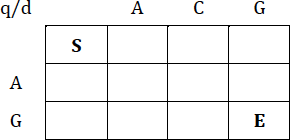
\includegraphics[width=0.3\textwidth]{fig02/alignment_to_table.png}
\end{figure}

\noindent \textbf{2. Add arrows}

We use three types of arrows to form an alignment.
\begin{itemize}
\item Move diagonally: add the letters from ‘q’ and ‘d’ to the alignment
\item Move vertically: add ‘-’ and the letter from ‘d’ to the alignment
\item Move horizontally: add the letter from ‘q’ and ‘-’ to the alignment
\end{itemize}

It shoud start from S and stops at E.

\begin{figure}[H]
  \centering
      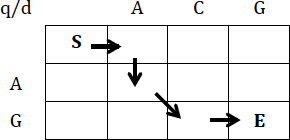
\includegraphics[width=0.3\textwidth]{fig02/alignment_to_table_example.png}
\end{figure}

%
% Exercise \thesection.3
%
\subsubsection*{Exercise \thesection.3}

Find the corresponding alignments for Table 1, 2 and 3.

\begin{multicols}{3}
Table 1
\begin{figure}[H]
  \centering
      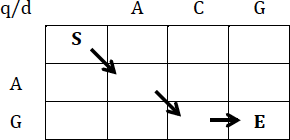
\includegraphics[width=0.3\textwidth]{fig02/alignment_to_table_exercise1.png}
\end{figure}

Table 2
\begin{figure}[H]
  \centering
      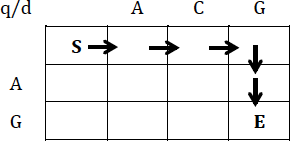
\includegraphics[width=0.3\textwidth]{fig02/alignment_to_table_exercise2.png}
\end{figure}

Table 3
\begin{figure}[H]
  \centering
      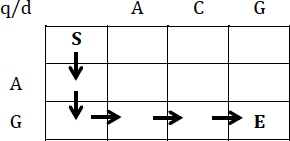
\includegraphics[width=0.3\textwidth]{fig02/alignment_to_table_exercise3.png}
\end{figure}

\end{multicols} 

%\end{document}


\end{document}


